\section{Soal}
Misalkan $a,b,c > 0$ dan memenuhi $a+b+c=1$. Tunjukkan bahwa
\begin{align*}
\dfrac{ab}{1+c}+\dfrac{bc}{1+a}+\dfrac{ca}{1+b} \le \dfrac{1}{4}.
\end{align*}

\newpage
\section{Komentar}
Oke, jadi beberapa hari lalu, aku ngepost soal yang sama dan secara "tersembunyi", menantang pemirsa untuk mencari dimana letak kesalahannya. Dan yap, 18 menit setelah dipost, udah ada yang nemu kesalahannya.

\begin{figure}[h]
    \centering
    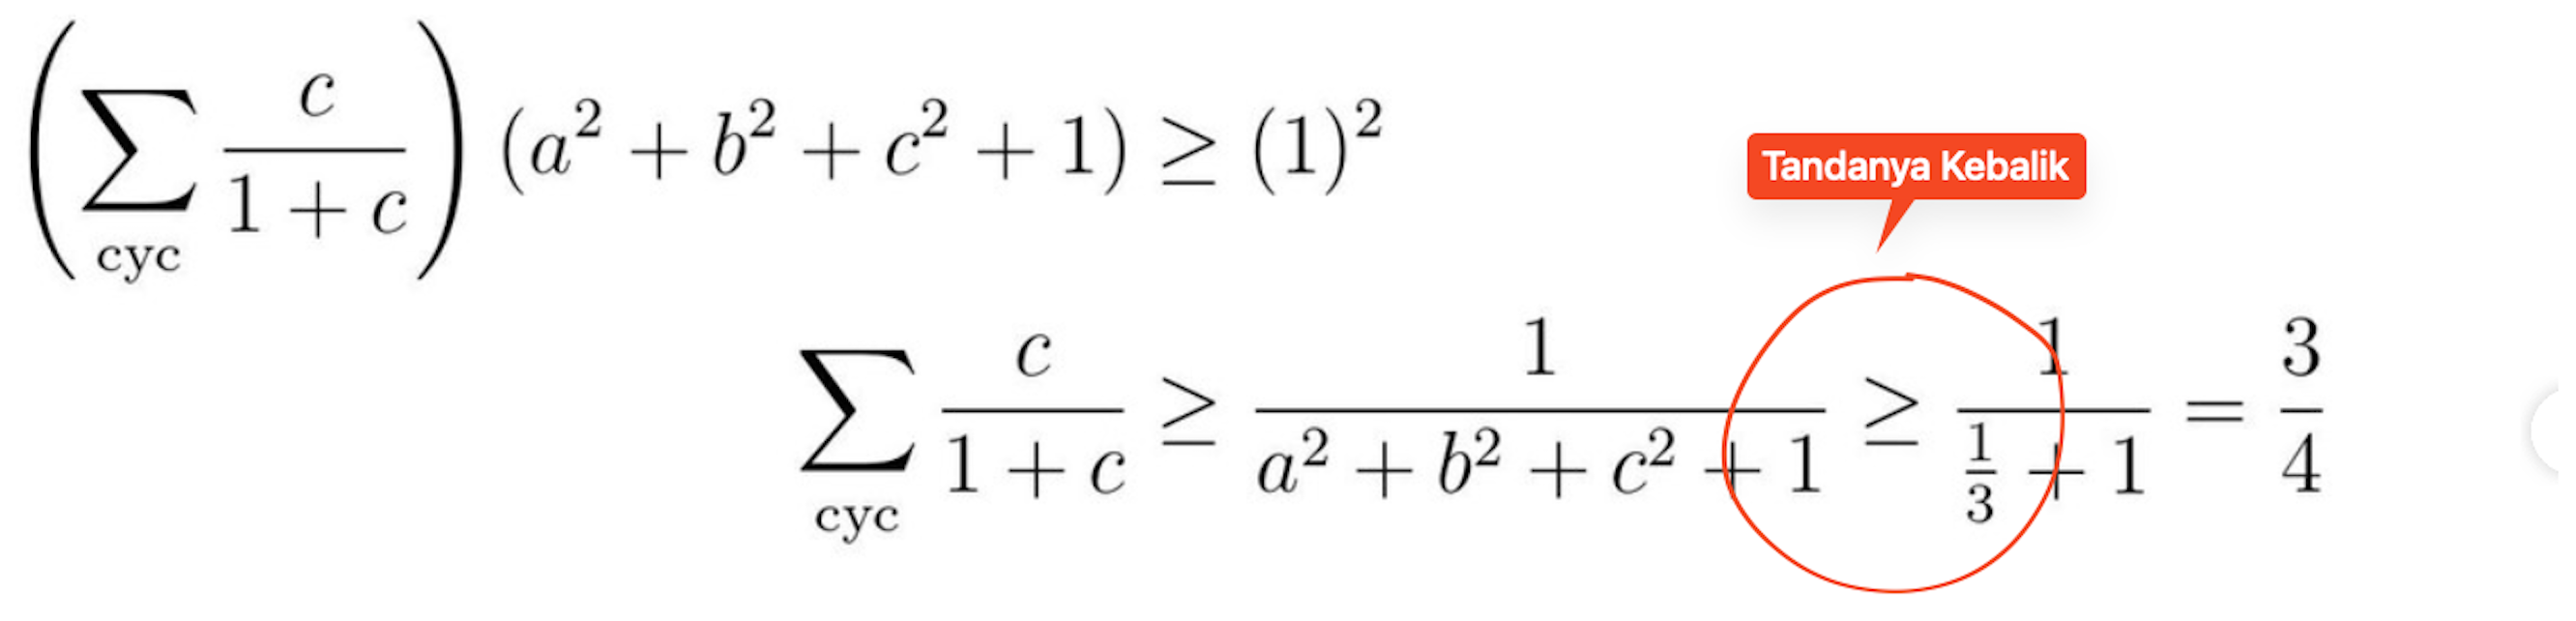
\includegraphics[scale=0.2]{18/redemption-mistake.png}
    \caption{\textbf{Kesalahan di post yang lalu (halaman kedua). Yes, tandanya kebalik.}}
\end{figure}

Nah, di post kali ini, niatnya aku mau redemption. Yes, tentu saja kasih solusi yang benernya.

\section{Motivasi - Walkthrough}
Oh iya, motivasi nemu solusinya darimana? Ya itu gunakan $1=a+b+c$. Kan di soalnya ada $\frac{ab}{1+c}$ gitu. Angka 1 nya agak "ganggu" ngga sih? Nah karena itu, coba disubstitusi $1=a+b+c$ ke penyebutnya dan coba pecah-pecah biar keliatan "simetrisnya"

\newpage
\section{Solusi}

    Perhatikan dengan Cauchy-Schwarz kita punya
    \begin{align*}
        \cycsum \dfrac{ab}{1+c} &= \cycsum \dfrac{ab}{a+b+2c}\\
        &= \cycsum \dfrac{ab}{(c+a)+(b+c)}\\
        &\le \cycsum \dfrac{ab}{(1+1)^2}\left(\dfrac{1}{a+c} + \dfrac{1}{b+c}\right)\\
        &= \dfrac{1}{4} \cycsum \left(\dfrac{ab}{a+c} + \dfrac{ab}{b+c}\right)\\
        &= \dfrac{1}{4}\cycsum \left(\dfrac{ab}{b+c}+\dfrac{ca}{b+c}\right)\\
        &= \dfrac{1}{4}\cycsum \dfrac{a(b+c)}{b+c}\\
        &= \dfrac{1}{4}\cycsum a\\
        &= \dfrac{1}{4}.
    \end{align*}
    dengan kesamaan saat $a=b=c$. Terbukti.
